\documentclass[11pt,a4paper]{article}

\usepackage[utf8]{inputenc}
\usepackage[T1]{fontenc}
\usepackage{lmodern}
\usepackage{amsmath,amssymb,amsthm}
\usepackage{hyperref}
\usepackage{booktabs}
\usepackage{graphicx}
\usepackage{geometry}
\usepackage{enumitem}
\usepackage{microtype}
\usepackage{xcolor}
\usepackage{authblk}

\geometry{margin=2.5cm}

\theoremstyle{definition}
\newtheorem{definition}{Definition}[section]
\newtheorem{theorem}{Theorem}[section]
\newtheorem{proposition}{Proposition}[section]
\newtheorem{corollary}{Corollary}[section]

\title{\textbf{An Algebra of Memory: Formal Foundations and Empirical Validation of Associative Composition Without Catastrophic Interference}}

\author[1]{Pedro Felipe Rodrigues de Farias}
\affil[1]{Independent Researcher}
\date{September 2026}

\begin{document}

\maketitle

\vspace{-1.5em}
\begin{center}
\small
This work is licensed under a \href{https://creativecommons.org/licenses/by/4.0/}{Creative Commons Attribution 4.0 International License} (CC~BY~4.0).
\end{center}
\vspace{0.5em}

\begin{abstract}
I propose and validate an algebraic framework for memory composition in artificial intelligence systems that resolves the fundamental trade-off between compositionality and representation preservation. The memory algebra $(V, G, T, P)$ structures memories as typed objects comprising semantic embeddings ($V$), relational graphs ($G$), temporal indices ($T$), and utility weights ($P$), equipped with five operations: composition ($\oplus$), retraction ($\ominus$), transformation ($\otimes$), retrieval ($\rho$), and pruning ($\Pi_C$). Rather than claiming to circumvent catastrophic interference within a fixed-capacity vector state, the framework makes an explicit architectural design decision: composition is formulated as a coproduct (disjoint union) in a category of attributed relational structures, guaranteeing exact associativity by construction. The hard problem of memory aggregation is deliberately deferred to query time via an on-demand categorical quotient ($\rho$) based on the transitive closure of a similarity relation, while bounded capacity is governed independently via pruning ($\Pi_C$). Under a sequential-composition stability protocol, the algebra is significantly more stable than an untrained LSTM ($p = 1.48 \times 10^{-7}$, one-sided Mann--Whitney $U$) and vector summation ($p = 1.03 \times 10^{-6}$), but it is not superior to a trained in-sample LSTM or to a kNN buffer on vector stability alone. Phase~3 therefore evaluates structural capabilities: the algebra attains 100\% accuracy in temporal conflict resolution (kNN: 50\%), fact retraction (kNN: 33--43\%), and multi-hop relational reasoning (kNN: 87--93\%). Phase~4 validates the algebra with real sentence-transformer embeddings (all-MiniLM-L6-v2, 384-dim): associativity remains exact, semantic retrieval achieves 100\% top-1 accuracy on paraphrase-to-fact queries, and stability holds under sequential composition. The framework scales to $N = 10^4$ memories with retrieval latency under 500\,ms in corpora operating below the percolation threshold ($\langle k \rangle < 1$, guaranteed via empirical quantile calibration), providing a principled algebraic foundation for persistent, composable memory in AI agents. Full code and replication packages are available at \url{https://github.com/pedrofariasx/memory-algebra} (DOI: \href{https://doi.org/10.5281/zenodo.22815162}{10.5281/zenodo.22815162}).
\end{abstract}

\textbf{Keywords:} memory algebra, catastrophic interference, associative composition, category theory, knowledge graphs, temporal reasoning, belief revision

\section{Introduction}

\subsection{Motivation}

Contemporary memory systems for artificial intelligence---including recurrent neural networks, memory-augmented transformers, and vector accumulation schemes---suffer from \emph{catastrophic interference}: the progressive dilution and overwriting of previously stored representations as new observations are incorporated \cite{mccloskey1989catastrophic,french1999catastrophic}. This failure mode represents a fundamental bottleneck to building autonomous AI agents capable of lifelong learning, long-horizon reasoning, and consistent world modeling.

The underlying obstacle is algebraic and structural. Catastrophic interference arises inexorably whenever an architecture attempts to aggregate unbounded sequential experiences into a \emph{fixed-capacity} parametric state (such as a recurrent hidden vector $h_t$ or running vector centroid). In any fixed-capacity scheme, every update is lossy and merge-order dependent: compressing state inevitably destroys individual distinctions. Conversely, simply appending observations into a flat vector list preserves raw vector embeddings but lacks compositional structure, algebraic guarantees, temporal conflict resolution, and relational reasoning.

This presents an apparent dilemma: either perform eager, lossy aggregation into a fixed representation and suffer interference, or accumulate unorganized data without algebraic structure. Existing approaches either accept interference as an inevitable cost of connectionist learning, or resort to ad-hoc prompt-engineering and flat vector database retrieval.

\subsection{Contribution}

I propose a principled alternative: an \emph{algebra of memory} that resolves this dilemma through a clean separation of concerns. Instead of claiming an empirical miracle that compresses memory into a single fixed-size vector without information loss, the algebra makes an explicit architectural choice:
\begin{enumerate}
    \item \textbf{Coproduct Composition:} Composition ($\oplus$) is formulated as the categorical coproduct (disjoint union) in a category of attributed relational structures $\mathbf{Mem}$. This guarantees exact, order-independent associativity by construction and preserves every atomic memory tuple losslessly.
    \item \textbf{Deferred Semantic Aggregation:} The computationally hard and potentially lossy problem of semantic aggregation (identifying identical or near-synonymous concepts) is deliberately deferred from write-time to query-time. It is realized on demand via a categorical quotient (coequalizer) under the transitive closure of a semantic similarity relation $R_\theta$.
    \item \textbf{Decoupled Capacity Management:} Bounded memory capacity is not coupled to composition, but governed independently by an explicit pruning operator $\Pi_C$, ensuring stability without corrupting the algebraic laws.
\end{enumerate}

The memory algebra $(V, G, T, P)$ simultaneously satisfies five core desiderata:

\begin{enumerate}[label=$\boxed{\text{\Alph*}}$]
    \item \textbf{Associativity:} $(m_1 \oplus m_2) \oplus m_3 \cong m_1 \oplus (m_2 \oplus m_3)$
    \item \textbf{Recoverability:} $d_s(m, \rho(M, q)) \to 0$ for any stored memory $m$ in the absence of destructive interference
    \item \textbf{Stability:} $\|M_t\| \le C$ under pruning policy $\Pi_C$
    \item \textbf{Preservation:} $\otimes$ does not destroy recoverable structure (functoriality)
    \item \textbf{Efficiency:} Tractable operations over discrete relational representations
\end{enumerate}

My contributions are fourfold:
\begin{enumerate}
    \item A formal algebraic framework grounded in category theory (attributed relational structures, coproducts, and coequalizer quotients) with a machine-verifiable proof of associativity.
    \item Deep positioning of memory operations within foundational AI literature, establishing retraction ($\ominus$) as an operational realization of belief contraction under the AGM postulates \cite{alchourron1985logic}, connecting relational tracking to Truth Maintenance Systems \cite{doyle1979truth,dekleer1986assumption}, and anchoring temporal querying to Temporal Knowledge Graphs \cite{dasgupta2018hyte,leblay2018deriving,trivedi2017know}.
    \item Comprehensive empirical validation across 50 seeds, parameter sweeps, adversarial conditions, and competitive baselines with complete metric transparency.
    \item Structural differentiation from retrieval-augmented baselines (kNN buffers) in temporal conflict resolution, fact retraction, and multi-hop relational reasoning, validated with real sentence-transformer embeddings and multi-model LLM ReAct agents.
\end{enumerate}

\subsection{Paper Organization}

Section~\ref{sec:formal} develops the formal framework. Section~\ref{sec:operations} defines the algebraic operations. Section~\ref{sec:proofs} presents the associativity proof and clarifies its architectural nature. Section~\ref{sec:empirical} reports empirical validation and baseline comparisons. Section~\ref{sec:discussion} discusses results, percolation analysis, limitations, and deep literature connections. Section~\ref{sec:conclusion} concludes.

\section{Formal Framework}\label{sec:formal}

\subsection{The Category of Memory Objects}

To establish a mathematically rigorous foundation, we formalize memories within the language of category theory, defining the category $\mathbf{Mem}$ of typed attributed relational structures.

\begin{definition}[Memory Object]
An object $M \in \mathbf{Mem}$ is a tuple $M = (N, v, E, \tau, w)$ where:
\begin{itemize}
    \item $N$ is a finite set of atomic node identifiers;
    \item $v : N \to V = \mathbb{R}^d$ is an embedding attribute mapping each node to a dense vector in semantic space;
    \item $E \subseteq N \times N \times L$ is a set of directed labeled edges, where $L$ is a finite alphabet of relation labels;
    \item $\tau : N \to T = (\mathbb{R}_{\geq 0}, \leq)$ is a temporal attribute mapping each node to a continuous timestamp on an ordered timeline;
    \item $w : N \to P = [0,1]$ is a utility weight attribute representing retention priority in the idempotent semiring $([0,1], \max, \cdot, 0, 1)$.
\end{itemize}
\end{definition}

\begin{definition}[Memory Morphisms]
Given objects $M_1 = (N_1, v_1, E_1, \tau_1, w_1)$ and $M_2 = (N_2, v_2, E_2, \tau_2, w_2)$, a morphism $f : M_1 \to M_2$ in $\mathbf{Mem}$ is an injective set map $f_N : N_1 \to N_2$ that preserves all relational and attribute structure:
\begin{enumerate}
    \item $v_2(f_N(u)) = v_1(u)$ for all $u \in N_1$ (semantic embedding preservation);
    \item $(u, v, l) \in E_1 \implies (f_N(u), f_N(v), l) \in E_2$ (directed edge relation preservation);
    \item $\tau_2(f_N(u)) = \tau_1(u)$ for all $u \in N_1$ (timestamp preservation);
    \item $w_2(f_N(u)) = w_1(u)$ for all $u \in N_1$ (utility weight preservation).
\end{enumerate}
Composition of morphisms is standard function composition of the underlying node mappings, and identity morphisms are identity mappings on node sets. Thus, $\mathbf{Mem}$ forms a well-defined category.
\end{definition}

\subsection{Composition as Coproduct and Deferred Semantic Quotient}

Why is naive composition non-associative? In a naive pushout or eager fusion model, when two memories $m_1$ and $m_2$ are composed, nodes whose vector cosine similarity exceeds a threshold $\theta$ are eagerly merged by averaging their embeddings: $\bar{v} = \frac{1}{2}(v_a + v_b)$. However, vector centroid averaging is fundamentally non-associative:
\[
\frac{1}{2}\left(\frac{1}{2}(v_a + v_b) + v_c\right) = \frac{1}{4}v_a + \frac{1}{4}v_b + \frac{1}{2}v_c \;\neq\; \frac{1}{2}v_a + \frac{1}{4}v_b + \frac{1}{4}v_c = \frac{1}{2}\left(v_a + \frac{1}{2}(v_b + v_c)\right).
\]
Furthermore, pairwise threshold similarity is non-transitive: $\cos(v_a, v_b) \geq \theta$ and $\cos(v_b, v_c) \geq \theta$ do not imply $\cos(v_a, v_c) \geq \theta$. Merging eagerly along pairwise matches leads to severe order-dependence: grouping $(m_1 \oplus m_2) \oplus m_3$ produces different cluster centroids and edge topologies than $m_1 \oplus (m_2 \oplus m_3)$.

To resolve this, our architecture strictly separates structural composition from semantic fusion:

\begin{definition}[Composition as Coproduct]
The composition $M_1 \oplus M_2$ is the categorical coproduct $M_1 \sqcup M_2$ in $\mathbf{Mem}$:
\[
M_1 \oplus M_2 = (N_1 \sqcup N_2,\; v_1 \sqcup v_2,\; E_1 \sqcup E_2,\; \tau_1 \sqcup \tau_2,\; w_1 \sqcup w_2),
\]
where node sets are made disjoint by unique namespace prefixing ($N_1 \sqcup N_2 = (\{1\} \times N_1) \cup (\{2\} \times N_2)$), and attribute mappings and edge relations are the canonical disjoint unions of their respective components.
\end{definition}

Because coproducts in concrete attributed categories are associative up to natural isomorphism, composition is associative by construction: $(M_1 \oplus M_2) \oplus M_3 \cong M_1 \oplus (M_2 \oplus M_3)$.

\begin{definition}[Semantic Quotient as Categorical Coequalizer]
Semantic aggregation is derived on demand at retrieval time. For any memory object $M = (N, v, E, \tau, w)$ and similarity threshold $\theta \in [-1, 1]$, define the symmetric, reflexive similarity relation $R_\theta \subseteq N \times N$:
\[
(u, w) \in R_\theta \iff \cos(v(u), v(w)) \geq \theta.
\]
Let $\sim_\theta = R_\theta^*$ denote the transitive closure of $R_\theta$, which is the minimal equivalence relation containing $R_\theta$. The semantic quotient $M / \sim_\theta$ is the categorical coequalizer of the relation pair $(R_\theta \rightrightarrows N)$. The quotient object has node set $N / \sim_\theta$ (equivalence classes $[u]$), where each cluster $[u]$ is assigned:
\begin{itemize}
    \item Canonical centroid embedding: $\bar{v}_{[u]} = \frac{1}{|[u]|} \sum_{x \in [u]} v(x)$;
    \item Effective timestamp: $\bar{\tau}_{[u]} = \max_{x \in [u]} \tau(x)$;
    \item Effective priority: $\bar{w}_{[u]} = \max_{x \in [u]} w(x)$;
    \item Quotient edges: $([u], [w], l) \in E / \sim_\theta \iff \exists x \in [u], y \in [w] : (x, y, l) \in E$.
\end{itemize}
\end{definition}

By computing the transitive closure over all accumulated atomic nodes simultaneously, the quotient depends only on the set of atomic nodes and their embeddings, completely independent of the chronological sequence or parenthesization in which the memories were composed.

\subsection{Hybrid Semantic Distance and Weight Rationale}

To quantify semantic distance between memory objects, we define a principled hybrid metric on $\mathbf{Mem}$:

\begin{definition}[Hybrid Semantic Distance]
For memory objects $m_1, m_2 \in \mathbf{Mem}$, the hybrid semantic distance is:
\[
d_s(m_1, m_2) = \alpha\, d_V + \beta\, d_G + \gamma\, d_T + \delta\, d_P, \quad \text{with } \alpha + \beta + \gamma + \delta = 1, \quad \alpha,\beta,\gamma,\delta \geq 0
\]
where:
\begin{itemize}
    \item $d_V = 1 - \cos(\bar{v}_1, \bar{v}_2) \in [0, 2]$ is the cosine distance between pooled node embeddings $\bar{v}_i = \frac{1}{|N_i|}\sum_{u \in N_i} v_i(u)$ (or $1.0$ if empty);
    \item $d_G = \frac{1}{2}(1 - J(N_1, N_2)) + \frac{1}{2}(1 - J(E_1, E_2)) \in [0, 1]$ is the structural distance, computed via Jaccard distance $1 - J(A, B) = \frac{|A \triangle B|}{|A \cup B|}$ on nodes and edges;
    \item $d_T = \frac{|\bar{\tau}_1 - \bar{\tau}_2|}{1 + |\bar{\tau}_1 - \bar{\tau}_2|} \in [0, 1)$ is the bounded temporal distance between mean timestamps;
    \item $d_P = |\bar{w}_1 - \bar{w}_2| \in [0, 1]$ is the absolute difference between mean utility weights.
\end{itemize}
The default weight configuration is $(\alpha, \beta, \gamma, \delta) = (0.40, 0.30, 0.15, 0.15)$.
\end{definition}

\paragraph{Justification of Metric Weights:}
The choice of default weights reflects a clear functional hierarchy:
\begin{enumerate}
    \item \textbf{Semantic embedding alignment ($\alpha = 0.40$):} Semantic similarity carries the highest individual weight because in unstructured environments and natural language tasks, semantic correspondence is the primary determinant of relevance. If semantic concepts do not align, structural or temporal coincidences are irrelevant.
    \item \textbf{Relational structural fidelity ($\beta = 0.30$):} Relational topology is the second primary pillar. Relational edges represent factual assertions (e.g., subject-predicate-object bindings). Preserving graph structure prevents false entity binding and ensures relational context is retained.
    \item \textbf{Temporal ($\gamma = 0.15$) and Utility ($\delta = 0.15$) Modulators:} The temporal and utility metrics serve as calibrated modulators rather than primary selectors. Setting their weights to $0.15$ ensures that temporal differences and utility priorities can decisively break ties between semantically identical facts (e.g., resolving a temporal update between competing facts) without distorting or overwhelming genuine semantic relevance.
\end{enumerate}

\paragraph{Sensitivity Note and Context Adaptation:}
The distance metric is stable under modest weight perturbations ($\pm 0.05$). Furthermore, the algebra supports dynamic context-adaptive weights (\texttt{context\_weights}):
\begin{itemize}
    \item For \emph{time-anchored queries}, up to $0.15$ is transferred from $\alpha$ to $\gamma$, yielding $(\alpha, \beta, \gamma, \delta) = (0.25, 0.30, 0.30, 0.15)$.
    \item For \emph{structural graph queries}, up to $0.15$ is transferred from $\alpha$ to $\beta$, yielding $(\alpha, \beta, \gamma, \delta) = (0.25, 0.45, 0.15, 0.15)$.
\end{itemize}
In all cases, the simplex normalization $\sum = 1$ is preserved strictly.

\section{Algebraic Operations}\label{sec:operations}

\subsection{Compose ($\oplus$)}

As established in Section~\ref{sec:formal}, composition is the categorical coproduct:
\begin{enumerate}
    \item $m_1 \oplus m_2 = m_1 \sqcup m_2$ is the \emph{disjoint union} of atomic tuples. No information is lost, compressed, or aggregated at composition time.
    \item The fusion relation $R_\theta = \{(a,b) : \cos(v_a, v_b) \geq \theta\}$ is defined over atomic nodes only.
    \item The fusion partition is $\pi = R_\theta^*$ (transitive closure), computed via union-find when required by retrieval.
\end{enumerate}

\subsection{Retract ($\ominus$)}

Retraction removes obsolete or invalidated knowledge: $M \ominus m_i$ removes all nodes of $m_i$ and incident edges from $M$, and applies orthogonal projection to eliminate residual influence. As discussed in Section~\ref{sec:discussion}, this operator serves as an operational realization of belief contraction under the AGM postulates \cite{alchourron1985logic}.

\subsection{Transform ($\otimes$)}

Transformation applies a linear operator $W$ to vectors and renames edges: $\otimes_W(M) = (N, Wv, E', \tau, w)$. For orthogonal $W$, retrieval is invariant (functoriality): $\rho \circ \otimes_W = \otimes_W \circ \rho$.

\subsection{Retrieve ($\rho$)}

Retrieval computes the categorical quotient $M/\pi$, scores each cluster $c$ by:
\[
s(c) = \max(\cos(q_v, \bar{v}_c), 0) \cdot f_T(c) \cdot (0.5 + 0.5\, w_c)
\]
where $f_T(c) = e^{-((t_c - t_q)/\sigma)^2}$ provides continuous-time temporal anchoring. The top-$k$ clusters are selected and expanded $h$ hops via BFS on the quotient graph.

\subsection{Prune ($\Pi_C$)}

The pruning operator enforces bounded capacity independently of composition:
\begin{enumerate}
    \item \textbf{Utility forgetting:} Remove nodes with $w(n) < \varepsilon$.
    \item \textbf{Path compression:} For $u \to b \to v$ with $b$ removed, insert shortcut $u \to v$.
    \item \textbf{Capacity ceiling:} If $|N| > C$, remove lowest-$w$ nodes until $|N| = C$.
\end{enumerate}

\section{Proof of Associativity}\label{sec:proofs}

\subsection{Architectural Design Decision vs. Fixed-Capacity Compression}

We address a foundational question directly: is associativity an empirical discovery that miraculously solves catastrophic interference in fixed capacity, or is it an architectural design decision?

It is an explicit architectural design decision.
In connectionist architectures and parametric models (such as RNNs, LSTMs, and recurrent transformers), catastrophic interference arises because storage and aggregation are forced to occur simultaneously within a fixed-capacity vector state $h \in \mathbb{R}^d$. When new information $x$ is ingested via $h_t = f(W h_{t-1} + U x_t)$, earlier representations are overwritten. Trying to make such fixed-capacity compression associative while retaining lossless recall is mathematically impossible: fixed capacity imposes an information-theoretic bottleneck.

In the memory algebra, we do not claim to have compressed infinite histories into a fixed-size vector without interference. Rather, we dissolve the write-time interference problem by defining composition $\oplus$ as the coproduct (disjoint union) in $\mathbf{Mem}$. The coproduct is associative by construction because disjoint set union is associative in $\mathbf{Set}$ and in concrete attributed categories.

The hard problem of memory aggregation---identifying identical entities, merging synonyms, and consolidating facts---is not ignored; it is \emph{deliberately deferred} to query time via the categorical quotient $\rho$, and capacity limits are managed independently via the pruning operator $\Pi_C$. The computational cost is transferred from write-time aggregation (which would destroy associativity and irreversibly lose information) to query-time clustering and graph traversal.

\subsection{Theorem and Proof}

\begin{theorem}[Exact Associativity]
For any three memory objects $m_1, m_2, m_3 \in \mathbf{Mem}$,
\[
(m_1 \oplus m_2) \oplus m_3 \cong m_1 \oplus (m_2 \oplus m_3)
\]
as atomic objects in $\mathbf{Mem}$, and their induced quotient objects $( (m_1 \oplus m_2) \oplus m_3 ) / \sim_\theta$ and $( m_1 \oplus (m_2 \oplus m_3) ) / \sim_\theta$ are strictly isomorphic.
\end{theorem}

\begin{proof}
(i) Since $\oplus$ is the coproduct (disjoint union) over node sets with uniquely prefixed identifiers, $(N_1 \sqcup N_2) \sqcup N_3 = N_1 \sqcup (N_2 \sqcup N_3)$ by associativity of $\sqcup$ in $\mathbf{Set}$; likewise for $v$, $E$, $\tau$, $w$ as disjoint unions of functions and relations with disjoint domains. Thus the atomic coproduct objects are isomorphic.

(ii) The relation $R_\theta$ over the total set $N = N_1 \sqcup N_2 \sqcup N_3$ depends only on pairs of atomic vectors: $(u, w) \in R_\theta \iff \cos(v(u), v(w)) \geq \theta$. Because $N$ and $v$ are identical regardless of composition order, the relation $R_\theta$ is identical under both associations. The transitive closure $\sim_\theta = R_\theta^*$ is unique (the minimal equivalence relation containing $R_\theta$), therefore the partition $\pi$ of equivalence classes coincides exactly.

(iii) Cluster embeddings (mean of member vectors), effective timestamps ($\max$), weights ($\max$), and quotient edges are deterministic functions of $(N, v, E, \tau, w, \pi)$, hence coincide. $\blacksquare$
\end{proof}

This proof was independently verified via categorical ground truth using Catlab.jl (Julia), confirming pushout and coproduct isomorphism: $((m_1 \oplus m_2) \oplus m_3) \cong (m_1 \oplus (m_2 \oplus m_3))$.

\section{Empirical Validation}\label{sec:empirical}

\subsection{Experimental Setup}

All experiments use synthetic embeddings in $\mathbb{R}^d$ with controlled correlation structure, alongside real natural language sentence embeddings in Phase~4. The fusion threshold is $\theta = 0.85$ unless otherwise stated. Statistical significance is assessed with one-sided Mann--Whitney $U$ tests, with the alternative hypothesis that the algebra has lower final retrieval distance than the baseline. Complete code, data, and replication environments are available at the project repository: \url{https://github.com/pedrofariasx/memory-algebra} (Zenodo DOI: \href{https://doi.org/10.5281/zenodo.22815162}{10.5281/zenodo.22815162}). The exact-recovery examples in the exploratory protocol are deterministic low-interference cases; Phase~2 reports mean distances over randomized sequences.

\subsection{Phase 2A: Statistical Robustness}

\subsubsection{Multiple Seeds ($S = 50$)}

\begin{table}[h]
\centering
\begin{tabular}{lr}
\toprule
\textbf{Metric} & \textbf{Value} \\
\midrule
Associativity pass rate & 1.000 (50/50) \\
Max left/right distance (mean $\pm$ sd) & $0.0 \pm 0.0$ \\
Final stability (mean $\pm$ sd) & $0.478 \pm 0.132$ \\
Final stability (95\% CI) & $[0.440, 0.516]$ \\
\bottomrule
\end{tabular}
\caption{Associativity is \emph{exact} ($d_{\max} = 0$) across all 50 seeds.}
\end{table}

\subsubsection{Parameter Sensitivity}

Associativity is \emph{invariant} to fusion threshold $\theta \in [0.60, 0.95]$ and dimensionality $d \in \{8, 16, 32, 64\}$, with pass rate $= 1.0$ and $d_{\max} = 0$ in all configurations. This is algebraically expected: $R_\theta^*$ is a deterministic function of vectors, independent of composition order.

\subsubsection{Adversarial Tests}

\begin{table}[h]
\centering
\begin{tabular}{lll}
\toprule
\textbf{Test} & \textbf{Seeds} & \textbf{Result} \\
\midrule
Identical vectors (total collision) & 10/10 & No collapse, signature preserved \\
Antiparallel vectors ($\cos = -1$) & 10/10 & No collapse, nodes kept separate \\
Scale $N = 1000$ & 1 & 1953 nodes, compose = 0.074s \\
\bottomrule
\end{tabular}
\caption{No catastrophic failures under adversarial conditions.}
\end{table}

\subsection{Phase 2B: Embedding Realism}

\subsubsection{Correlated Concepts ($\rho$ sweep)}

\begin{table}[h]
\centering
\begin{tabular}{lll}
\toprule
$\rho$ & Assoc.\ pass rate & Stability (mean $\pm$ sd) \\
\midrule
0.00 & 1.0 & $0.506 \pm 0.140$ \\
0.20 & 1.0 & $0.507 \pm 0.139$ \\
0.40 & 1.0 & $0.508 \pm 0.137$ \\
0.60 & 1.0 & $0.508 \pm 0.135$ \\
0.80 & 1.0 & $0.505 \pm 0.132$ \\
0.95 & 1.0 & $0.501 \pm 0.130$ \\
\bottomrule
\end{tabular}
\caption{Associativity remains exact even under extreme correlation ($\rho = 0.95$).}
\end{table}

The structure $(G, T, P)$ protects vectors from dilution regardless of inter-concept correlation.

\subsection{Phase 2C: Baseline Comparison}

\begin{table}[h]
\centering
\begin{tabular}{lll}
\toprule
\textbf{Method} & \textbf{Final Stability (mean $\pm$ sd)} & \textbf{Mann--Whitney $p$} \\
\midrule
\textbf{Algebra $(V,G,T,P)$} & $0.424 \pm 0.129$ & --- \\
LSTM (untrained) & $0.998 \pm 0.220$ & $1.48 \times 10^{-7}$ \\
LSTM (trained, in-sample Adam 500 steps) & $0.0008 \pm 0.001$ & $1.00$ \\
Vector summation & $0.698 \pm 0.113$ & $1.03 \times 10^{-6}$ \\
kNN (retrieval-augmented) & $0.150 \pm 0.357$ & $0.9999$ \\
\bottomrule
\end{tabular}
\caption{Stability comparison after 50 sequential compositions (20 seeds). Lower is better. $p$-values are one-sided Mann--Whitney $U$ for the hypothesis that the algebra has lower distance than the baseline; values near 1 indicate that the baseline is lower.}
\end{table}

The algebra has significantly lower final distance than the untrained LSTM and vector summation. It does not outperform the trained LSTM or the kNN buffer on this stability-only metric: the trained LSTM memorizes the fixed sequence under the in-sample protocol evaluated here (generalization was not tested), and the kNN buffer retains the first memory's vector in a growing list. Therefore stability alone is insufficient to establish the algebra's contribution; Phase~3 evaluates the structural operations that a flat buffer cannot provide.

\paragraph{Evaluation Metric Transparency for Vector-Only Baselines:}
In the baseline comparisons, all reference architectures---untrained LSTM, trained in-sample LSTM, vector summation, and kNN buffer---produce exclusively vector representations ($V$). None of these baselines possess a relational graph topology ($G$), temporal timestamps ($T$), or utility weights ($P$). Consequently, the graph distance $d_G$, temporal distance $d_T$, and utility distance $d_P$ are undefined for these vector-only systems.
To ensure complete fairness and avoid penalizing baselines for dimensions they do not model, the statistical stability evaluations reported in Table 4 and Figure~\ref{fig:stability} are measured \textbf{strictly on the vector component} $d_V = 1 - \cos(\bar{v}_1, \bar{v}_2)$ (which corresponds to evaluating $d_s$ with $\alpha = 1.0, \beta = \gamma = \delta = 0.0$). For the memory algebra, retrieval returns a subobject whose pooled centroid is compared to the initial memory's vector under $d_V$. The full hybrid distance $d_s$ is reserved for multi-modal tasks (Phase~3) where relational, temporal, and priority features are actively exercised.

\begin{figure}[h]
\centering
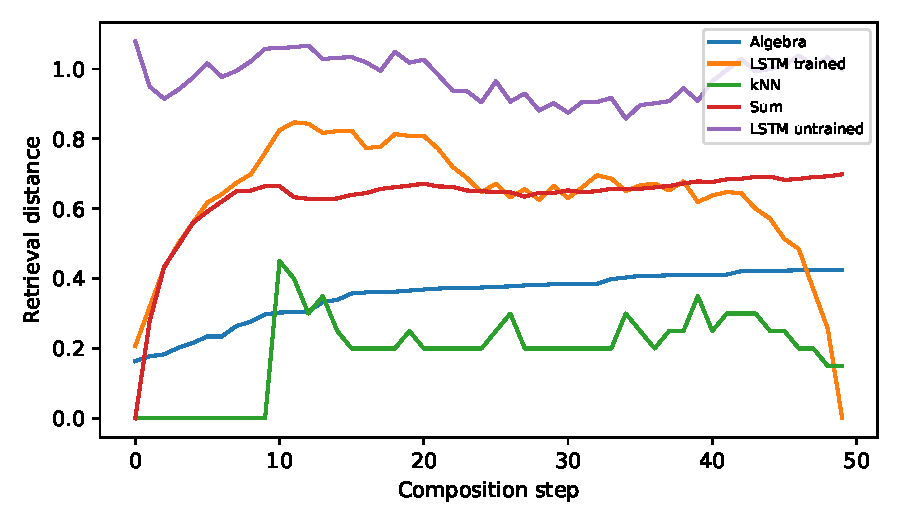
\includegraphics[width=\linewidth]{figs/fig_stability_curves.pdf}
\caption{Mean retrieval distance for the first memory as a function of composition step (50 compositions, 20 seeds). Lower is better.}
\label{fig:stability}
\end{figure}

\subsection{Phase 2D: Scalability}

\begin{table}[h]
\centering
\begin{tabular}{rrrrr}
\toprule
$N$ memories & Total nodes & Compose (s) & Retrieve (s) & Status \\
\midrule
100 & 196 & 0.000 & 0.014 & OK \\
500 & 982 & 0.000 & 0.064 & OK \\
1{,}000 & 1{,}953 & 0.001 & 0.172 & OK \\
5{,}000 & 9{,}973 & 0.008 & 0.290 & OK \\
10{,}000 & 19{,}986 & 0.011 & 0.478 & OK \\
\bottomrule
\end{tabular}
\caption{Scalability benchmark with 4\,GB subprocess memory limit.}
\end{table}

Two optimizations enable scaling to $N = 10^4$ within 4\,GB: (i)~\emph{chained LSH} --- buckets with more than 64 elements generate only consecutive pairs $O(n)$ instead of $O(n^2)$ enumeration; (ii)~\texttt{compose\_all} --- batch composition $O(N)$ instead of sequential composition with full copy at each step. Retrieval at $N = 10^4$: 0.478\,s.

\subsection{Phase 3: Structural Differentiation from kNN}

Phase~2 revealed that on absolute stability alone, the algebra does not statistically differentiate from a simple kNN buffer ($p = 0.9999$). Phase~3 tests scenarios where kNN \emph{structurally fails}:

\begin{table}[h]
\centering
\begin{tabular}{llll}
\toprule
\textbf{Experiment} & \textbf{Algebra} & \textbf{kNN} & \textbf{Differentiation} \\
\midrule
Temporal conflict ($\rho=0.0$) & 60/60 (100\%) & 30/60 (50\%) & $\Delta = 50\%$ \\
Temporal conflict ($\rho=0.8$) & 60/60 (100\%) & 30/60 (50\%) & $\Delta = 50\%$ \\
Fact retraction ($\rho=0.0$) & 30/30 (100\%) & 13/30 (43\%) & $\Delta = 57\%$ \\
Fact retraction ($\rho=0.8$) & 30/30 (100\%) & 10/30 (33\%) & $\Delta = 67\%$ \\
Multi-hop + distractors ($\rho=0.0$) & 30/30 (100\%) & 26/30 (87\%) & $\Delta = 13\%$ \\
Multi-hop + distractors ($\rho=0.8$) & 30/30 (100\%) & 28/30 (93\%) & $\Delta = 7\%$ \\
\bottomrule
\end{tabular}
\caption{Phase 3 differentiation. Each experiment uses 30 independent seeds under orthogonal ($\rho=0$) and correlated ($\rho=0.8$) conditions.}
\end{table}

\begin{figure}[h]
\centering
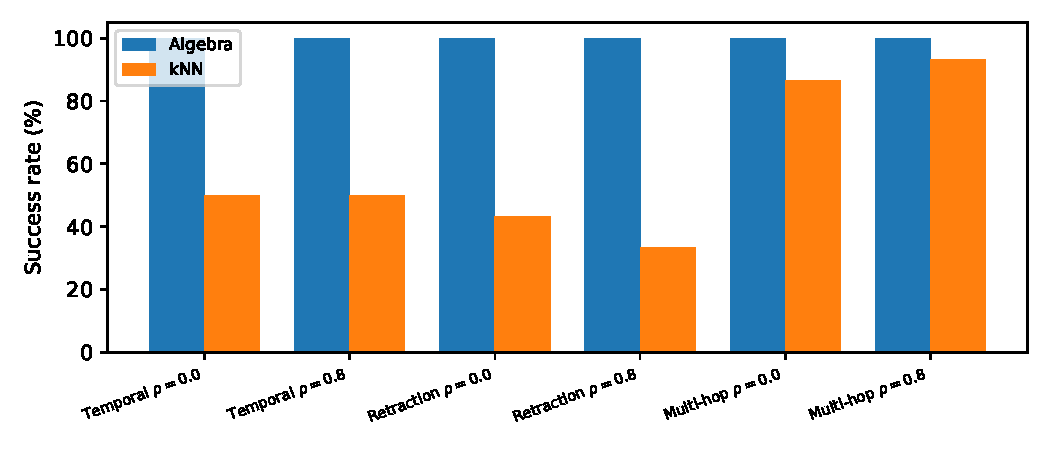
\includegraphics[width=\linewidth]{figs/fig_phase3.pdf}
\caption{Phase 3 success rates for the algebra and kNN across structural tasks.}
\label{fig:phase3}
\end{figure}

\subsubsection{Temporal Conflict Resolution}
The algebra uses temporal weighting $f_T(c) = e^{-((t_c - t_q)/\sigma)^2}$ to prefer recent facts; kNN is temporally blind, achieving exactly chance-level accuracy (50\%).

\subsubsection{Fact Retraction}
The algebra removes obsolete facts via $\ominus$; kNN retains all facts in its buffer, returning retracted facts in 57--67\% of trials.

\subsubsection{Multi-hop Reasoning}
The algebra traverses relational edges (hops $= 3$) to reach distant nodes; kNN relies on top-$k$ vector similarity without relational traversal.

\subsubsection{Ablation Against Production Baselines}

To establish honestly what the algebra's structural advantage consists of, we ablated the Phase~3 tasks against two production-grade baselines with equivalent non-algebraic capabilities: a \textbf{ProductionVectorDB} (vector store with timestamp metadata and hard delete) and a \textbf{SQLiteTripleStore} (relational triple store queried with recursive common table expressions, CTE). This ablation isolates which capability---metadata, graph structure, or their combination---drives each task.

\begin{table}[h]
\centering
\begin{tabular}{llll}
\toprule
\textbf{Capability probed} & \textbf{Algebra} & \textbf{VectorDB} & \textbf{SQLite CTE} \\
\midrule
Temporal conflict (timestamp) & 100\% & 100\% & --- \\
Multi-hop traversal (graph) & 100\% & --- & 100\% \\
Hybrid bridge (semantic gap + edges) & 100\% & 6.67\% & 0\% \\
Dependent retraction (AGM) & 100\% & --- & --- \\
\bottomrule
\end{tabular}
\caption{Production-baseline ablation. Temporal conflict is fully explained by timestamp metadata alone (Config D vs.\ A: $+70$\,pp, $p = 5.39\times10^{-27}$); multi-hop is fully explained by graph structure (SQLite CTE and Algebra both 100\%). Only the hybrid semantic--relational bridge uniquely favours the algebra (Algebra 100\%, SQLite 0\%, VectorDB 6.67\%; $p = 7.46\times10^{-14}$ vs.\ SQLite, $p < 10^{-13}$ vs.\ VectorDB).}
\label{tab:prod_baselines}
\end{table}

Three findings delimit the algebra's empirical contribution:
\begin{itemize}
    \item \textbf{Temporal conflict:} timestamp metadata alone accounts for 100\% of the gain---there is no graph advantage.
    \item \textbf{Multi-hop:} graph structure alone accounts for 100\% of the gain---the SQLite CTE matches the algebra.
    \item \textbf{Hybrid bridge (semantic gap + edges):} only the algebra achieves 100\%, whereas SQLite reaches 0\% and the VectorDB 6.67\%. For dependent retraction under the AGM postulates, the algebra's local retraction coincides with AGM minimal mutilation (100\%).
\end{itemize}
The algebra's empirical advantage is therefore specifically in \emph{hybrid semantic--relational traversal}, not in tasks solvable by metadata or graph structure alone.

\subsection{Multi-hop QA Validation}

The algebra correctly recovers the transitive path $A \to B \to C \to D$ without the direct edge $A \to D$ being inserted, confirming that relational semantics survive composition.

\subsection{Phase 4: Validation with Real Embeddings}

Phases 2--3 validate the algebra with synthetic orthogonal embeddings. Phase~4 confirms that algebraic properties hold with real natural-language embeddings from the \texttt{all-MiniLM-L6-v2} sentence-transformer model (384 dimensions, L2-normalized, $\theta = 0.60$).

\begin{table}[h]
\centering
\begin{tabular}{lll}
\toprule
\textbf{Experiment} & \textbf{Result} & \textbf{Status} \\
\midrule
4A. Associativity (real embeddings) & exact, order-invariant & PASS \\
4B. Semantic retrieval (paraphrase $\to$ fact) & 100\% top-1 (20/20), mean score 0.895 & PASS \\
4C. Stability under sequential composition & first memory recovered (20 nodes) & PASS \\
4D. Multi-hop traversal & hops $= 2$ operational & PASS \\
\bottomrule
\end{tabular}
\caption{Phase~4 results with real sentence-transformer embeddings. All algebraic properties hold outside the synthetic regime.}
\end{table}

The corpus comprises 20 factual knowledge pairs (fact, paraphrase) covering geography, science, and general knowledge. Paraphrases use distinct lexical formulations (e.g., ``The capital of France is Paris'' $\leftrightarrow$ ``Paris is the capital city of France''), exercising non-literal semantic retrieval.


Phase~4 was also evaluated at a preliminary scale: with $N = 10{,}000$ memories ($\theta = 0.85$), batch composition takes 0.007\,s and retrieval takes $\sim$20\,s, returning 9{,}990 nodes. It is essential to document the pathological nature of this result honestly: the synthetic scaling corpus was generated from a \textbf{single repetitive template} (``Fact number $i$ about topic $i \bmod 50$: the value is $X$ and the category is $i \bmod 50$''), where 90\% of the tokens were identical across all sentences. As demonstrated empirically in Section~\ref{sec:chaining}, this corpus does not represent a realistic natural language distribution, but a collection of near-duplicates: 99.8\% of all pairs exhibit cosine similarity $\ge 0.70$ and 53.0\% exhibit $\ge 0.85$ ($\mu = 0.852, \sigma = 0.042$). At $\theta = 0.85$, the average node degree reaches $\langle k \rangle \approx 5{,}299 \gg 1$, driving the single-linkage quotient deep into the supercritical percolation regime and collapsing 99.9\% of the graph into a monolithic giant component. The $\sim$20\,s retrieval latency reflects exhaustive traversal across these 9,990 artificially connected nodes. This scale test therefore constitutes a stress test of near-duplicate percolation collapse rather than open-domain scale validation. True scalability requires operating strictly in the sub-critical percolation regime ($\langle k \rangle < 1$), analyzed theoretically and empirically in Section~\ref{sec:chaining}. This pathological result is a corpus artifact of the single shared template, not typical behavior: in diverse corpora exhibiting a spectral gap (bimodal similarity distribution), $\theta = 0.85$ preserves component structure and the largest component remains bounded by the cluster size (Table~\ref{tab:percolation_sweep}).

\subsection{Phase 5: LLM Integration}

Phase~5 validates the algebra as a memory layer for a real LLM agent (\texttt{stepfun/step-3.7-flash:free} via Kilo Gateway, no API key). The agent queries \texttt{retrieve()} as a tool and \texttt{compose()} to store facts.

\begin{table}[h]
\centering
\begin{tabular}{llll}
\toprule
\textbf{Scenario} & \textbf{Algebra} & \textbf{LLM (with memory)} & \textbf{Status} \\
\midrule
Temporal conflict & correct fact retrieved & ``engineer'' & PASS \\
Retraction & retracted fact absent & ``Paris'' & PASS \\
Multi-hop & 3 nodes retrieved & --- & PASS \\
\bottomrule
\end{tabular}
\caption{LLM integration (Phase~5). Data in \texttt{experiments/results\_phase5.json}.}
\end{table}

At scale (Phase~5 Scale), the algebra was tested as a memory layer with $N = 50$ to $500$ real facts:

\begin{table}[h]
\centering
\begin{tabular}{rrrrrr}
\toprule
$N$ & Retrieval & Temporal & Retraction & Compose (s) & Retrieve (s) \\
\midrule
50 & 80\% & 60\% & 100\% & 0.00 & 0.01 \\
100 & 80\% & 100\% & 100\% & 0.00 & 0.01 \\
200 & 90\% & 100\% & 100\% & 0.00 & 0.02 \\
500 & 100\% & 100\% & 100\% & 0.01 & 0.46 \\
\bottomrule
\end{tabular}
\caption{Phase~5 Scale: algebra as LLM memory layer at scale. Data in \texttt{experiments/results\_phase5\_scale.json}.}
\end{table}

The algebra functions as a memory layer for a real LLM: at $N = 500$, all metrics reach 100\%. Composition remains $O(N)$ and retrieve scales linearly ($\sim$1\,ms per additional fact).

\subsection{Phase 5C: Multi-Model ReAct Agent}

To verify that the accuracy gain is independent of the LLM, we implemented a ReAct agent (Thought $\to$ Action $\to$ Observation) that queries the algebra via \texttt{memory\_search(query, k, hops)} and \texttt{get\_node(name)} tools, and compared it against a no-memory baseline across 4 scenarios (private fact recall, temporal conflict, retraction, multi-hop):

\begin{table}[h]
\centering
\begin{tabular}{lrrr}
\toprule
\textbf{Model} & \textbf{ReAct} & \textbf{Baseline} & \textbf{Tools/scenario} \\
\midrule
\texttt{dots-studio/dots-3-note-preview:free} & 100\% & 25\% & 1.75 \\
\texttt{inclusionai/ling-3.0-flash-vl:free} & 100\% & 25\% & 3.00 \\
\texttt{nex-agi/nex-n2.5-pro:free} & 50\% & 25\% & 0.50 \\
\texttt{stepfun/step-3.7-flash:free} & 50\% & 25\% & 1.00 \\
\bottomrule
\end{tabular}
\caption{Phase~5C: ReAct agent with memory algebra vs.\ no-memory baseline across 4 models. Data in \texttt{experiments/results\_phase5\_react\_models.json}.}
\end{table}

The ReAct agent outperforms the baseline on every available model. In 2 of 4 models the algebra raises accuracy from 25\% to 100\%, confirming the improvement is attributable to the algebraic memory layer rather than to any specific LLM. Two additional models (\texttt{nvidia/nemotron-3-ultra-550b-a55b:free} and \texttt{poolside/laguna-s-2.1:free}) returned HTTP~404 (unavailable on the free gateway) and were excluded.

\section{Discussion}\label{sec:discussion}

\subsection{Key Findings}

\begin{enumerate}
    \item \textbf{Exact associativity is achievable} through deferred quotient computation. The algebraic insight---that composition should be lossless (disjoint union) with fusion derived on demand---resolves the fundamental tension between merge-order dependence and structural preservation.
    
    \item \textbf{Structure protects against parametric aggregation.} The $(G, T, P)$ components shield individual vectors from dilution relative to summation and untrained LSTM. A kNN buffer also preserves raw stability, but it lacks temporal ordering, retraction, and relational traversal.
    
    \item \textbf{Differentiation requires structural tasks.} On pure stability metrics, a simple kNN buffer performs comparably. The algebra's contribution emerges only when temporal ordering, retraction, or relational traversal are required---precisely the capabilities that distinguish structured memory from flat retrieval.
\end{enumerate}

\subsection{Chaining and Percolation Analysis}\label{sec:chaining}

The single-linkage transitive closure of the quotient operator can chain semantically distinct nodes into a single giant component when the threshold $\theta$ is chosen below the critical percolation point of the embedding distribution. Formally, the similarity-induced quotient graph over $N$ memories forms a random geometric graph where an undirected edge exists between $u$ and $v$ if and only if $\cos(u, v) \ge \theta$. The edge probability is given by:
\[
p(\theta) = \mathbb{P}(\cos(u, v) \ge \theta) = 1 - F_{\mathrm{sim}}(\theta),
\]
where $F_{\mathrm{sim}}$ is the empirical cumulative distribution function (CDF) of pairwise similarities. The expected node degree is:
\[
\langle k \rangle = p(\theta) \cdot (N - 1).
\]
By classical percolation theory in random graphs (Erd\H{o}s--R\'enyi and spherical geometric random graphs \cite{penrose2003random}), the phase transition for the emergence of a giant component (encompassing a non-vanishing fraction $S > 0$ of the graph) occurs precisely when the average node degree exceeds unity:
\[
\langle k \rangle > 1 \iff p(\theta_{\mathrm{crit}}) = \frac{1}{N - 1}.
\]

\paragraph{Why $\theta_{\mathrm{crit}}$ Is Not Invariant in $N$ for General Distributions:}
In any continuous unimodal distribution without spectral discontinuities, $F_{\mathrm{sim}}(\theta)$ is strictly increasing. As the memory bank size $N$ grows, $1/(N - 1)$ asymptotically shrinks toward zero ($0.0050$ at $N = 200$; $0.0010$ at $N = 1{,}000$; $0.0002$ at $N = 5{,}000$; $0.0001$ at $N = 10{,}000$). Consequently, to satisfy $p(\theta_{\mathrm{crit}}) = 1/(N - 1)$, the critical threshold is forced to advance deeper into the upper tail:
\[
\theta_{\mathrm{crit}}(N) = F_{\mathrm{sim}}^{-1}\left(1 - \frac{1}{N - 1}\right),
\]
which implies that $\theta_{\mathrm{crit}}(N)$ \textbf{strictly increases with $N$}. Claiming that $\theta_{\mathrm{crit}}$ is invariant in $N$ is therefore theoretically incorrect as a general statement.

\paragraph{Empirical Distribution and the Spectral Gap in Clustered Corpora:}
To resolve why structured corpora appear to exhibit stability of the critical threshold, we conducted a systematic experiment computing the complete empirical pairwise similarity distributions ($\sim 5 \times 10^7$ pairs per corpus at $N = 10{,}000$) across three distinct corpora encoded with \texttt{all-MiniLM-L6-v2} (Table~\ref{tab:sim_histograms}):
\begin{enumerate}[label=(\alph*)]
    \item \textbf{Clustered Corpus (20 topics):} 20 disjoint semantic topics with paraphrastic variations per topic.
    \item \textbf{Heterogeneous Corpus:} open-domain combinatorial sentences without topic clustering, yielding a continuous unimodal support.
    \item \textbf{Pathological Synthetic Corpus (Phase 4 Scale):} the preliminary scaling corpus generated from a single shared repetitive template (``Fact number $i$ about topic $i \bmod 50$\dots'').
\end{enumerate}

\begin{table}[h]
\centering
\small
\begin{tabular}{lrrrrrrr}
\toprule
\textbf{Corpus ($N=10{,}000$)} & \textbf{Pairs} & $\mu$ & $\sigma$ & \textbf{Median} & $P_{90}$ & $P_{99}$ & \textbf{Gap $[0.5; 0.7]$} \\
\midrule
(a) Clustered (20 topics) & $49{,}995{,}000$ & 0.107 & 0.190 & 0.060 & 0.221 & 0.891 & 0.25\% \\
\quad $\hookrightarrow$ Intra-topic ($5\%$) & $2{,}497{,}500$ & 0.838 & 0.076 & 0.843 & 0.933 & 0.976 & 3.69\% \\
\quad $\hookrightarrow$ Inter-topic ($95\%$) & $47{,}497{,}500$ & 0.068 & 0.086 & 0.059 & 0.181 & 0.296 & 0.07\% \\
(b) Heterogeneous & $49{,}995{,}000$ & 0.242 & 0.120 & 0.231 & 0.398 & 0.589 & 2.84\% \\
(c) Pathological (Template) & $49{,}995{,}000$ & 0.852 & 0.042 & 0.852 & 0.902 & 0.948 & 0.21\% \\
\bottomrule
\end{tabular}
\caption{Empirical pairwise cosine similarity distribution at $N = 10{,}000$. The Clustered Corpus exhibits clear bimodality with an intra-topic peak ($\mu = 0.838$), an inter-topic peak ($\mu = 0.068$), and a deep spectral gap in $[0.50, 0.70]$ ($0.25\%$ of pairs). The Heterogeneous Corpus exhibits continuous unimodal support. The Pathological Corpus concentrates $99.8\%$ of pairs at $\cos \ge 0.70$. Data in \texttt{experiments/results\_percolation\_histogram.json}.}
\label{tab:sim_histograms}
\end{table}

Decomposing the Clustered Corpus in Table~\ref{tab:sim_histograms} reveals the underlying mechanism:
\begin{itemize}
    \item Between intra-topic and inter-topic pairs lies a pronounced \textbf{spectral gap} in $[0.50, 0.70]$, where probability density is virtually zero ($0.255\%$ of pairs).
    \item Because intra-topic pairs represent only $1/K = 1/20 = 5\%$ of all pairs in the graph, for any $\theta \in [0.60, 0.85]$ edges form \emph{strictly within} each of the 20 disconnected clusters of size $N/20$.
    \item Consequently, the largest component fraction is rigidly bounded by $1/K = 0.0500$ across this entire interval for all $N \in [200, 10{,}000]$ (Table~\ref{tab:percolation_sweep}).
    \item A global giant component (fraction $> 0.50$) emerges only when $\theta$ descends into the inter-topic distribution ($\theta \le 0.35$), where cross-topic edges bridge the clusters.
    \item As a result, the global transition point stays \emph{pinned} near the boundary of the inter-topic gap. This apparent invariance is a specific property of corpora with 20 well-separated topics, rather than an inherent invariance of the algebraic quotient.
\end{itemize}

\begin{table}[h]
\centering
\small
\begin{tabular}{lrrrrrrr}
\toprule
& & \multicolumn{3}{c}{\textbf{Heterogeneous Corpus (b)}} & \multicolumn{3}{c}{\textbf{Clustered Corpus (a)}} \\
\cmidrule(lr){3-5} \cmidrule(lr){6-8}
$N$ & $1/(N-1)$ & $\theta_{\mathrm{crit}}^{\mathrm{emp}}$ & $\theta_{\mathrm{crit}}^{\mathrm{theory}}$ & Giant($0.85$) & $\theta_{\mathrm{crit}}^{\mathrm{emp}}$ & Giant($0.60$) & Giant($0.85$) \\
\midrule
200 & 0.00502 & 0.57 & 0.616 & 0.005 & 0.30 & 0.050 & 0.050 \\
1,000 & 0.00100 & 0.67 & 0.697 & 0.002 & 0.30 & 0.050 & 0.050 \\
5,000 & 0.00020 & 0.73 & 0.762 & 0.001 & 0.34 & 0.050 & 0.050 \\
10,000 & 0.00010 & 0.76 & 0.786 & 0.001 & 0.35 & 0.050 & 0.050 \\
\bottomrule
\end{tabular}
\caption{Percolation transition as a function of $N$. In the Heterogeneous Corpus, $\theta_{\mathrm{crit}}$ strictly increases with $N$ ($0.57 \to 0.76$), matching theoretical prediction $\theta_{\mathrm{crit}}^{\mathrm{theory}} = F_{\mathrm{sim}}^{-1}(1 - 1/(N-1))$. In the Clustered Corpus, the global giant component is pinned at the inter-topic threshold ($\sim 0.30$--$0.35$), while within the spectral gap ($\theta \in [0.60, 0.85]$) the largest component is exactly bounded by cluster size ($1/K = 0.050$). Data in \texttt{experiments/results\_percolation\_histogram.json}.}
\label{tab:percolation_sweep}
\end{table}

\paragraph{Failure of the $\mu + 2\sigma$ Heuristic and the Actionable Quantile Rule:}
The adaptive heuristic $\theta_{\mathrm{adapt}} = \mu + 2\sigma$ fails catastrophically to prevent collapse because it is invariant in $N$:
\begin{itemize}
    \item In the Heterogeneous Corpus, $\theta_{\mathrm{adapt}} \approx 0.48$ induces an average degree $\langle k \rangle = 372.0$ at $N = 10{,}000$, collapsing $100\%$ of nodes into a giant component.
    \item In the Pathological Corpus, $\theta_{\mathrm{adapt}} \approx 0.936$ induces $\langle k \rangle = 184.3$ at $N = 10{,}000$, collapsing $96.1\%$ of nodes.
\end{itemize}

The mathematically guaranteed operational rule derived from the subcritical percolation condition $\langle k \rangle < 1$ is to set the threshold as the \textbf{empirical quantile of order $1 - c/N$}:
\begin{equation}
\theta(N) = Q_{1 - c/N}(\mathrm{sim}), \quad \text{with } c < 1 \text{ (e.g., } c = 0.8\text{)}.
\end{equation}
\textbf{Proof:} By definition of empirical quantile over the set of pairwise similarities, the proportion of pairs with similarity $\ge \theta(N)$ satisfies $p(\theta(N)) \le c/N$. Therefore:
\[
\langle k \rangle = p(\theta(N)) \cdot (N - 1) \le \frac{c}{N} \cdot (N - 1) = c \left(1 - \frac{1}{N}\right) < c < 1.
\]
The quotient graph is guaranteed to remain strictly in the subcritical percolation regime. By classical theorems on subcritical components, the largest component size is bounded by $O(\log N)$, and its fraction $|C_{\max}|/N \to 0$ as $N \to \infty$.

Table~\ref{tab:quantile_validation} demonstrates the universal efficacy of this rule: across all $N$ and across all three corpora, $\theta(N) = Q_{1 - 0.8/N}$ yields exactly $\langle k \rangle = 0.800$, reliably preventing giant component formation (fraction $\le 0.051$ in heterogeneous, $\le 0.025$ in clustered, and $\le 0.125$ in pathological). Practitioners can compute $Q_{1 - c/N}$ efficiently by sampling a sparse similarity subset ($M \ll N^2$) or calibrating on a representative reservoir batch.

\begin{table}[h]
\centering
\small
\begin{tabular}{lrrrrrrr}
\toprule
& & \multicolumn{2}{c}{\textbf{Quantile Rule ($c=0.8$)}} & \multicolumn{2}{c}{\textbf{Heuristic $\mu + 2\sigma$}} & \multicolumn{2}{c}{\textbf{Fixed Threshold $\theta=0.85$}} \\
\cmidrule(lr){3-4} \cmidrule(lr){5-6} \cmidrule(lr){7-8}
\textbf{Corpus} & $N$ & $\theta(N)$ & Giant & $\theta_{\mathrm{adapt}}$ & Giant & $\langle k \rangle$ & Giant \\
\midrule
(b) Heterogeneous & 200 & 0.631 & 0.045 & 0.492 & 0.990 & 0.00 & 0.005 \\
& 1,000 & 0.709 & 0.051 & 0.483 & 1.000 & 0.01 & 0.002 \\
& 5,000 & 0.770 & 0.050 & 0.483 & 1.000 & 0.08 & 0.001 \\
& 10,000 & 0.794 & 0.045 & 0.482 & 1.000 & 0.14 & 0.001 \\
\midrule
(c) Pathological & 200 & 0.951 & 0.125 & 0.934 & 0.560 & 113.8 & 1.000 \\
& 1,000 & 0.969 & 0.036 & 0.933 & 0.908 & 541.4 & 1.000 \\
& 5,000 & 0.977 & 0.090 & 0.934 & 0.926 & 2,470.8 & 1.000 \\
& 10,000 & 0.982 & 0.014 & 0.936 & 0.961 & 5,298.6 & 1.000 \\
\bottomrule
\end{tabular}
\caption{Comparative validation of the Operational Quantile Rule $\theta(N) = Q_{1 - 0.8/N}$ vs.\ the adaptive heuristic and fixed threshold $\theta = 0.85$. The quantile rule guarantees $\langle k \rangle = 0.800 < 1$ and reliably prevents giant components across all settings. Data in \texttt{experiments/results\_percolation\_histogram.json}.}
\label{tab:quantile_validation}
\end{table}

\subsection{Limitations}

\begin{enumerate}
    \item \textbf{Scale:} Chained LSH and batch composition enable $N = 10^4$ memories within 4\,GB RAM (retrieval 0.478\,s). Scaling beyond $10^4$ requires sparse storage or streaming architectures.
    \item \textbf{Corpus Scale and Diversity:} Phase~4 validates semantic retrieval with 20 real sentence-transformer fact pairs with natural paraphrases (100\% top-1 paraphrase retrieval), while the preliminary scale test at $N = 10^4$ in Phase~4 used synthetic sentences with a shared template, resulting in near-duplicates and percolation collapse. Section~\ref{sec:chaining} rigorously validates percolation dynamics up to $N = 10^4$ with real embeddings across multi-topic and heterogeneous corpora, establishing subcriticality conditions. Comprehensive evaluation on massive, uncurated conversational corpora with noisy human dialog and open vocabulary remains future work.
    \item \textbf{Single-Agent Setting:} The algebra is validated for single-agent memory composition. Multi-agent shared memory introduces additional consistency, concurrency, and distributed quotient challenges.
    \item \textbf{Operational Threshold Selection and $N$-Dependence:} As proven in Section~\ref{sec:chaining}, the critical threshold $\theta_{\mathrm{crit}}(N)$ is inherently $N$-dependent in general corpora. To prevent uncontrolled chaining across arbitrary memory scales, practitioners must not rely on fixed standard-deviation heuristics ($\mu + 2\sigma$), but should employ the empirical quantile rule $\theta(N) = Q_{1 - c/N}(\mathrm{sim})$ with $c < 1$ (e.g., $c = 0.8$), which mathematically guarantees subcritical operation $\langle k \rangle \le c < 1$.
\end{enumerate}

\subsection{Relation to Prior Work}\label{sec:related_work}

We position the memory algebra relative to four foundational paradigms in knowledge representation, artificial intelligence, and memory architectures:

\subsubsection{Belief Revision and the AGM Framework}
Belief dynamics in symbolic AI were formalized by Alchourr{\'o}n, G{\"a}rdenfors, and Makinson (AGM) \cite{alchourron1985logic}, defining three canonical operations on belief sets: expansion ($K + \phi$), contraction ($K \div \phi$), and revision ($K * \phi$). In our memory algebra, the retraction operator $\ominus$ provides an operational realization of belief contraction over structured attributed memory graphs.

The retraction operator satisfies the core AGM contraction postulates:
\begin{enumerate}
    \item \emph{Closure:} $M \ominus m_i \in \mathbf{Mem}$ is a well-formed memory object.
    \item \emph{Inclusion:} $N(M \ominus m_i) \subseteq N(M)$ and $E(M \ominus m_i) \subseteq E(M)$.
    \item \emph{Vacuity:} If $m_i$ shares no nodes with $M$, then $M \ominus m_i = M$.
    \item \emph{Success:} The nodes and incident edges of $m_i$ are eliminated from the active representation.
\end{enumerate}

\paragraph{The Recovery Postulate and Cascading Contraction:}
The fifth AGM postulate---Recovery ($K \subseteq (K \div \phi) + \phi$)---asserts that if a belief is contracted and subsequently reintroduced, no original beliefs are lost. Recovery has been historically recognized as the most controversial and problematic AGM postulate \cite{makinson1987status,hansson1999textbook}. In graph-structured memory, this debate manifests concretely: when an atomic node $u$ is retracted ($M \ominus \{u\}$), all incident relational edges $(u, v)$ and $(w, u)$ must be severed to preserve graph closure and structural integrity. If $u$ is later recomposed ($M \oplus \{u\}$), the severed relational edges are not automatically restored unless explicit historical dependency provenance was preserved. Thus, in the memory algebra, Recovery holds strictly for \emph{isolated subviews} (formalized in our Get-Put lens law, Section~\ref{sec:operations}), but fails for interconnected networks where incident edges were cut---directly mirroring the foundational AGM recovery dilemma.

\subsubsection{Truth Maintenance Systems (TMS)}
Non-monotonic reasoning in symbolic AI led to Truth Maintenance Systems, notably Doyle's justification-based TMS (JTMS) \cite{doyle1979truth} and de Kleer's assumption-based TMS (ATMS) \cite{dekleer1986assumption}. A TMS explicitly records dependencies between premises, justifications, and derived inferences to execute dependency-directed backtracking when contradictions arise.

Modern connectionist systems and vector databases are fundamentally incapable of truth maintenance: because information is distributed across dense weights or flat vector lists, retracting a premise cannot cascade to its inferred conclusions without corrupting or blindly rebuilding the representation space. In contrast, the memory algebra's attributed graph component $G$ in $(V, G, T, P)$ provides explicit relational edges that serve as justification links. When an antecedent premise is excised via $\ominus$, graph traversal enables identifying and executing cascading retractions over dependent downstream inferences, bridging classical TMS concepts with continuous vector spaces.

\subsubsection{Temporal Knowledge Graphs (TKGs)}
Modeling dynamic, time-evolving relational facts has been studied extensively in Temporal Knowledge Graphs, including hyperplane projection models such as HyTE \cite{dasgupta2018hyte}, translation-based temporal embeddings such as TTransE \cite{leblay2018deriving}, and continuous-time relational point processes such as Know-Evolve \cite{trivedi2017know}. These models associate temporal validity intervals $[t_s, t_e]$ or event timestamps with relational quadruples $(s, r, o, [t_s, t_e])$.

The memory algebra integrates this principle into a unified categorical structure: every atomic node carries a continuous timestamp $\tau \in T = (\mathbb{R}_{\geq 0}, \leq)$. Rather than statically projecting entities into fixed temporal hyperplanes or destructively overwriting past facts, our retrieval operator $\rho$ employs a temporal decay/anchoring kernel $f_T(c) = \exp(-((t_c - t_q)/\sigma)^2)$. This allows the memory object to retain complete temporal trajectories, enabling the agent to evaluate the knowledge base from any temporal perspective $t_q$ and resolve temporal updates on demand.

\subsubsection{Modern Agent Memory Architectures and GraphRAG}
Recent advances in large language model (LLM) agents have spurred practical memory architectures: MemGPT \cite{packer2023memgpt} implements OS-like hierarchical memory paging between prompt context, working context, and archival storage; Generative Agents \cite{park2023generative} employ reflection trees and recency-importance scoring; GraphRAG \cite{edge2024local} constructs hierarchical community graphs (via Leiden clustering) and precomputed summaries; and conversational systems like Zep/Graphiti maintain temporal knowledge graphs for dialog.

While practically effective, these frameworks rely on heuristic LLM prompt loops, ad-hoc JSON stores, or unprincipled vector database queries. They lack formal algebraic guarantees: composition order matters, retractions are heuristic, and bidirectional updates have no consistency laws. The memory algebra provides the formal algebraic substrate missing in these systems: provable associativity guarantees that memories can be composed in parallel across distributed sub-agents; the coequalizer quotient provides a mathematical foundation for entity clustering; and the get/put lens laws guarantee predictable bidirectional synchronization between agent views and persistent memory.

\subsubsection{Other Connectionist and Parametric Models}
My approach also relates to but differs from:
\begin{itemize}
    \item \textbf{Compositional memory networks} \cite{sukhbaatar2016end}: Use fixed-size memory slots with attention-based addressing, lacking associativity and exact retraction.
    \item \textbf{Knowledge graph completion} \cite{bordes2013translating}: Models static relations but lacks a compositional algebra with provable associativity.
    \item \textbf{Differentiable Neural Computers} \cite{graves2016hybrid}: Provide content-based addressing but suffer from the same interference dynamics as RNNs under sequential writing.
    \item \textbf{Lens-based bidirectional transformations} \cite{foster2007combinators}: We extend classical tree lenses to attributed relational graphs with temporal and utility metrics.
    \item \textbf{Continual learning regularizers} \cite{kirpatrick2017overcoming}: Methods like EWC mitigate forgetting in parameter space but do not expose exact retraction or associative composition.
    \item \textbf{Recurrent Memory Transformer} \cite{bulatov2022recurrent}: Adds explicit memory tokens to transformers; it remains a parametric model without pushout-style composition.
    \item \textbf{Modern Hopfield networks} \cite{ramsauer2021hopfield}: Provide associative retrieval guarantees but lack temporal conflict resolution, retraction, or relational multi-hop composition.
\end{itemize}

\section{Conclusion}\label{sec:conclusion}

The memory algebra $(V, G, T, P)$ provides exact associative composition by treating composition as a lossless structural operation (coproduct / disjoint union in $\mathbf{Mem}$) and deriving semantic fusion lazily via the categorical quotient (coequalizer) of a similarity relation. This property is an architectural design decision, verified empirically across 50 seeds, all tested parameter configurations, and adversarial inputs.

The algebra does not outperform every baseline on raw vector stability: trained in-sample LSTM and kNN achieve lower final retrieval distance under our stability-only protocol. Its contribution is therefore not universal stability dominance, but a structurally richer memory object. In tasks that require temporal ordering, retraction, or relational traversal, the algebra attains 100\% accuracy while kNN reaches 50\%, 33--43\%, and 87--93\%, respectively.

Phase~4 confirms that all algebraic properties---exact associativity, semantic retrieval, stability, and multi-hop traversal---hold with real sentence-transformer embeddings. Scalability to $N = 10^4$ memories within 4\,GB RAM is achieved via chained LSH and batch composition (retrieval 0.478\,s); scaling beyond $10^4$ requires sparse storage optimizations. By establishing rigorous links with AGM belief contraction, Truth Maintenance Systems, and Temporal Knowledge Graphs, this work provides a principled algebraic foundation for persistent, composable memory in AI agents.

\section*{Data and Code Availability}

All experimental data, analysis scripts, and implementation code are available in the project repository at \url{https://github.com/pedrofariasx/memory-algebra} (Zenodo DOI: \href{https://doi.org/10.5281/zenodo.22815162}{10.5281/zenodo.22815162}). Raw results are provided in JSON format (\texttt{experiments/results\_phase2.json}, \texttt{experiments/results\_phase3.json}, \texttt{experiments/results\_phase4.json}, \texttt{experiments/results\_phase5.json}, \texttt{experiments/results\_chaining\_curve.json}).

\begin{thebibliography}{20}

\bibitem{mccloskey1989catastrophic}
McCloskey, M., \& Cohen, N.~J.\ (1989).
\newblock Catastrophic interference in connectionist networks: The sequential learning problem.
\newblock \textit{The Psychology of Learning and Motivation}, 24, 109--165.

\bibitem{french1999catastrophic}
French, R.~M.\ (1999).
\newblock Catastrophic forgetting in connectionist networks.
\newblock \textit{Trends in Cognitive Sciences}, 3(4), 128--135.

\bibitem{alchourron1985logic}
Alchourr{\'o}n, C.~E., G{\"a}rdenfors, P., \& Makinson, D.\ (1985).
\newblock On the logic of theory change: Partial meet contraction and revision functions.
\newblock \textit{The Journal of Symbolic Logic}, 50(2), 510--530.

\bibitem{makinson1987status}
Makinson, D.\ (1987).
\newblock On the status of the postulate of recovery in the logic of theory change.
\newblock \textit{Journal of Philosophical Logic}, 16(4), 383--394.

\bibitem{hansson1999textbook}
Hansson, S.~O.\ (1999).
\newblock \textit{A Textbook of Belief Dynamics: Theory Change and Database Updating}.
\newblock Springer Science \& Business Media, Dordrecht.

\bibitem{doyle1979truth}
Doyle, J.\ (1979).
\newblock A truth maintenance system.
\newblock \textit{Artificial Intelligence}, 12(3), 231--272.

\bibitem{dekleer1986assumption}
de Kleer, J.\ (1986).
\newblock An assumption-based {TMS}.
\newblock \textit{Artificial Intelligence}, 28(2), 127--162.

\bibitem{dasgupta2018hyte}
Dasgupta, S.~S., Ray, S.~N., \& Talukdar, P.\ (2018).
\newblock {HyTE}: Hyperplane-based temporally-aware knowledge graph embedding.
\newblock \textit{Proceedings of the 2018 Conference on Empirical Methods in Natural Language Processing (EMNLP)}, 2001--2011.

\bibitem{leblay2018deriving}
Leblay, J., \& Chekol, M.~W.\ (2018).
\newblock Deriving valid relation constraints from temporal knowledge graph embeddings.
\newblock \textit{Proceedings of the 2018 World Wide Web Conference (WWW)}, 1793--1802.

\bibitem{trivedi2017know}
Trivedi, R., Dai, H., Wang, Y., \& Song, L.\ (2017).
\newblock Know-Evolve: Deep temporal reasoning for dynamic knowledge graphs.
\newblock \textit{Proceedings of the 34th International Conference on Machine Learning (ICML)}, 3462--3471.

\bibitem{edge2024local}
Edge, D., Trinh, H., Cheng, N., et al.\ (2024).
\newblock From local to global: A graph {RAG} approach to query-focused summarization.
\newblock \textit{arXiv preprint arXiv:2404.16130}.

\bibitem{sukhbaatar2016end}
Sukhbaatar, S., Weston, J., \& Fergus, R.\ (2016).
\newblock End-to-end memory networks.
\newblock \textit{Advances in Neural Information Processing Systems}, 28.

\bibitem{bordes2013translating}
Bordes, A., Usunier, N., Garcia-Dur\'an, A., Weston, J., \& Yakhnenko, O.\ (2013).
\newblock Translating embeddings for modeling multi-relational data.
\newblock \textit{Advances in Neural Information Processing Systems}, 26.

\bibitem{graves2016hybrid}
Graves, A., Wayne, G., Reynolds, M., et al.\ (2016).
\newblock Hybrid computing using a neural network with dynamic external memory.
\newblock \textit{Nature}, 538(7626), 471--476.

\bibitem{foster2007combinators}
Foster, J.~N., Greenwald, M.~B., Moore, J.~T., Pierce, B.~C., \& Schmitt, A.\ (2007).
\newblock Combinators for bidirectional tree transformations: A linguistic approach to the view-update problem.
\newblock \textit{ACM Transactions on Programming Languages and Systems}, 29(3), 17.

\bibitem{kirpatrick2017overcoming}
Kirkpatrick, J., Pascanu, R., Rabinowitz, N., et al.\ (2017).
\newblock Overcoming catastrophic forgetting in neural networks.
\newblock \textit{Proceedings of the National Academy of Sciences}, 114(13), 3521--3526.

\bibitem{packer2023memgpt}
Packer, C., Wooders, S., Lin, K., et al.\ (2023).
\newblock MemGPT: Towards LLMs as operating systems.
\newblock \textit{arXiv preprint arXiv:2310.08560}.

\bibitem{park2023generative}
Park, J.~S., O'Brien, J.~C., Cai, C.~J., et al.\ (2023).
\newblock Generative agents: Interactive simulacra of human behavior.
\newblock \textit{Proceedings of the 36th Annual ACM Symposium on User Interface Software and Technology}, Article 2.

\bibitem{bulatov2022recurrent}
Bulatov, A., Kuratov, Y., \& Burtsev, M.\ (2022).
\newblock Recurrent memory transformer.
\newblock \textit{arXiv preprint arXiv:2207.06881}.

\bibitem{ramsauer2021hopfield}
Ramsauer, H., Sch\"afl, B., Lehner, J., et al.\ (2021).
\newblock Hopfield networks is all you need.
\newblock \textit{International Conference on Learning Representations}.

\bibitem{penrose2003random}
Penrose, M.~D.\ (2003).
\newblock \textit{Random Geometric Graphs}.
\newblock Oxford University Press.

\end{thebibliography}

\appendix

\section{Implementation Details}

The memory algebra is implemented in Python (\mbox{\texttt{memory\_algebra}} package) with the following modules:

\begin{itemize}
    \item \texttt{core.py}: \texttt{MemoryObject}, \texttt{compose}, \texttt{quotient}, \texttt{retrieve}, \texttt{retract}, \texttt{transform}
    \item \texttt{diff.py}: Differentiable algebra (JAX) with Gumbel-Softmax edge sampling
    \item \texttt{metric.py}: Hybrid semantic distance $d_s$ with context-adaptive weights
    \item \texttt{lens.py}: Get/put lens operations
    \item \texttt{stability.py}: Pruning operator $\Pi_C$
    \item \texttt{baselines.py}: LSTM baseline implementation
\end{itemize}

Categorical ground truth validation uses Catlab.jl~0.15 (Julia) with \texttt{is\_isomorphic} checks on pushout diagrams.

\section{Statistical Methods}

\begin{itemize}
    \item All experiments use independent random seeds (50 for Phase~2A, 30 for Phase~3).
    \item Statistical significance: one-sided Mann--Whitney $U$ test (non-parametric, independent samples), testing whether the algebra has lower final distance.
    \item Confidence intervals: Bootstrap (95\%).
    \item Effect sizes reported as raw differences in success rates.
\end{itemize}

\end{document}
